\DiaryEntry{Nonlinear Dynamics and Chaos, 2}{2015-11-01}{Maths}

\subsubsection{Conservative System}

Based on Newton's law that $F=ma$. If a particle moves alone the x-axis and is subject to a non-linear force $F(x)$, we have

\[m \frac{d^2x(t)}{dt^2} = F(x)\]

Note the independence of $F(x)$ on both the derivative of $x(t)$ and the time $t$ itself.

If $V(x)$ denotes the potential energy $F(x) = - dV(x)/dx$, we have

\[m \frac{d^2x(t)}{dt^2} + \frac{dV(x)}{dx} = 0\]

If we multiply both sides of the equation with $dx(t)/dt$, we obtain

\[m \frac{dx(t)}{dt} \frac{d^2 x(t)}{dt^2} + \frac{dx(t)}{dt} \frac{dV(x)}{dx} = 0\]

The left part can be rewritten as

\[
\frac{d}{dt} \left[ \frac{1}{2} m \left(\frac{dx(t)}{dt}\right)^2 \right] = \frac{1}{2} m \frac{d^2 x(t)}{dt^2} 2 \frac{dx(t)}{dt} = m \frac{dx(t)}{dt} \frac{d^2 x(t)}{dt^2}
\]

the right part is (inverse chain rule)

\[
\frac{dx(t)}{dt} \frac{dV(x)}{dx} = \frac{dV(x)}{dt}
\]

We therefore have

\[
\frac{d}{dt} \left( \frac{1}{2} m \left(\frac{dx(t)}{dt}\right)^2 + V(x) \right) = 0
\]

This means that the total energy $E = \frac{1}{2} x'^2 + V(x)$ is constant for any solution of the system. In other words, the energy $E$ stays constant along trajectories.

\subsubsection{Limit Cycles}

A limit cycle is an isolated closed trajectory. Isolated means that nearby trajectories are not closed and spiral either toward (stable limit cycles) or away from the limit cycle (instable limit cycles). An example of a stable limit cycle and an unstable limit cycle are shown below.

\begin{figure}[H]
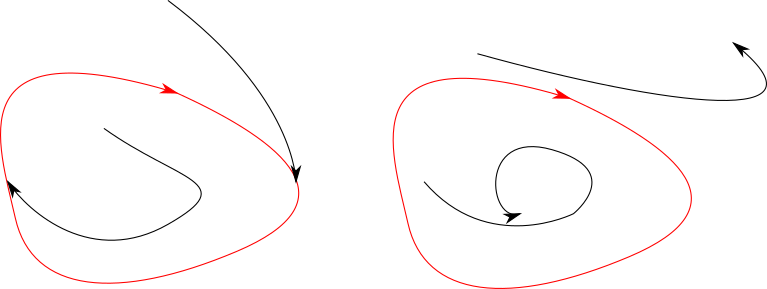
\includegraphics[scale=0.7]{images/strogatz_2_1.png}
\end{figure}

\subsection{Poincaré-Bendixon Theorem}

If

\begin{itemize}
\item
  R is a closed bounded subset of a plane
\item
  the system is continuously differentiable on R
\item
  R does not contain any fixed points
\item
  there is a trajectory C confined to R (i.e.~it stays within R for from $t=0$ till $t \rightarrow \infty$),
\end{itemize}

then C is a closed orbit or it spirals towards a closed orbit as
$t \rightarrow \infty$. In any case, R contains a closed orbit.

We can interpret the theorem that the dynamical possibilities of \textbf{two- dimensional} systems are limited. If a trajectory is confined to a closed, bounded region without fixed points, it must eventually approach a closed orbit. In higher-order dimensions, the theorem does not hold; therefore chaos (more ``dynamic'' behavior is
possible).
